\chapter{Testování a vyhodnocení výsledků}
\label{testovani-a-vyhodnoceni}

Oproti učení s~učitelem, kde je trénován model, jemuž často bývá přiřazena procentuální úspěšnost správného rozpoznávání díky anotovaným datům, učení bez učitele žádné takové měřítko neudává. Výsledek není s~čím porovnat, a~proto není možné jasně a číselně validovat výstup. Úkol dále ztěžuje objektivita pohledu na~to, co vůbec anomálií je. Ve~výsledku je tedy nutné, aby každý případ posoudil člověk a vyhodnotil, zda detekce proběhla v~pořádku. Jednotlivé sekce této kapitoly popisují, jak se řešení detekce anomálií testovalo a jaké závěry z~toho vyplynuly.

\section{Testování detekce anomálií v~délkách zpracování požadavků}
\label{testovani-delka-pozadavku}
Aby bylo možné testovat odhalení co nejvíce typů anomálií, bylo potřeba vytvořit dataset odpovídající reálným datům. V~něm pak šlo anomálie vytvářet a ověřovat, zda-li budou detekovány. Prvním způsobem testování bylo vytváření konkrétních dat a anomálií s~cílem vyzkoušení detekce anomálií nad~jejich různými typy. Druhým pak bylo náhodné generování provozu s~anomáliemi, jež se měly odhalovat.

\subsection{Vytvoření a nalezení konkrétní anomálie}
\label{testovani-konkretni-anomalie}
Smyslem tohoto testování bylo ověření schopnosti detekovat co nejvíce typů anomálií. Umožňovalo cíleně vytvářet anomálie různých velikostí, hustot či tvarů. Právě tento způsob testování nejvíce přispěl k~nalezení co nejobecnějších parametrů detekčních algoritmů. Odhaloval jak pozitiva, tak nedostatky hodnot určitých parametrů pro~jeden či druhý typ anomálie, což vedlo ke~kvalitnímu kompromisu.

Dataset se vytvářel následujícím způsobem. Platná data se vždy vygenerovala z~normálního, Fisher-Snedecorova nebo trojúhelníkového rozložení s~parametry odpovídajícími účelům konkrétního testu. Z~rovnoměrného rozložení přesahujícího hranice platných dat se následně vygenerovaly náhodné outliery. Anomálie se poté vytvářely na místech, kde se chtělo otestovat, jestli se tam naleznou. Testovaly se případy, kdy anomálie byly:

\begin{itemize}
  \item velikostí na~hranici limitu nebo naopak skoro stejně velké jako platná data,
  \item různé hustoty a tedy rozptylu, ať už velmi úzké nebo široké,
  \item odlišných rozložení (rovnoměrné, normální, Fisher-Snedecorovo, trojúhelníkové) různých parametrů,
  \item blízko platných dat nebo s~odstupem,
  \item větších počtů, kde se pak všechny vyskytovaly na~stejné straně od~platných dat, z~obou stran, nebo se anomálie navzájem i překrývaly.
\end{itemize}

Chyby nalezené během tohoto testování vedly na~úpravy parametrů detekčních algoritmů. Bylo proto prováděno, dokud se vyskytovaly chyby v~detekci, jež bylo možné odstranit. Testování dovedlo detekci do~stavu, ve~kterém je schopna rozpoznat téměř každou anomálii vytvořenou tímto způsobem. Neodstranitelným nedostatkem nalezeným tímto testováním se ukázala být občasná mylná klasifikace přirozených outlierů jako anomálie. Tento problém však nenastává při použití parametru tolerance anomálií v~určité vzdálenosti od~platných dat.

\subsection{Generování náhodného provozu}
Výše zmíněné testování by šlo zpochybnit tím, že se anomálie úspěšně detekovaly proto, že byly vytvářeny vlastnoručně. Z~toho důvodu a taktéž pro~testování ve~větším měřítku se detekce ověřovala i na~náhodných datech. Ta byla generována podobně jako u~předchozího přístupu a ze~stejných rozložení, neboť tak data v~RQA vypadají. Náhodnost spočívala ve~velikosti, tvaru a pozic jak platných, tak anomálních dat. Pseudokód \ref{pseudokod-generovani-provozu} velmi zjednodušeně popisuje tvorbu datasetu náhodného provozu.

\makeatletter
\renewcommand*{\ALG@name}{Algoritmus}
\makeatother
\begin{algorithm}
    \begin{algorithmic}[1]
    \STATE $pocet\gets Random(100, 5000)$
    \STATE $typRozlozni\gets NahodnyTypRozlozeni()$
    \STATE $rozlozeni\gets RozlozeniSNahodnymiParametry(pocet, typRozlozeni)$
    \STATE $pocetOutlieru\gets Random(0.5, 3)\cdot0.01\cdot pocet$
    \STATE $outliery\gets RovnomerneRozlozeni(pocetOutlieru, rozlozeni.RozsirenaOblast)$
    \STATE $volneOblasti\gets VypoctiVolneOblasti(rozlozeni, outliery)$
    \STATE $pocetAnomalii\gets 1$
    \STATE $pocetAnomaliiPom\gets Random(0, 1)$
    
    \IF{$pocetAnomaliiPom \leq 0.1$}
        \STATE $pocetAnomalii\gets 0$
      \ELSIF{$pocetAnomaliiPom \geq 0.9$}
        \STATE $pocetAnomalii\gets 2$
     \ENDIF
    
    \STATE $anomalie\gets List()$
    \FOR{$(i=0$; $i < pocetAnomalii$; $i\gets i+1)$}
        \STATE $oblast\gets volneOblasti[Random(0, len(volneOblasti)-1]$
        \STATE $velikost\gets Random(7.5, 12.5)\cdot0.01\cdot(pocet + pocetOutlieru)$
        \STATE $typ\gets NahodnyTypRozlozeni()$
        \STATE $anomalniRozlozni\gets RozlozeniSNahodnymiParametry(velikost, typ, oblast)$
        \STATE $anomalie.Add(anomalniRozlozni)$
    \ENDFOR
    \STATE $provoz\gets Shuffle(rozlozeni, outliery, anomalie)$
    \end{algorithmic}
    \caption{Pseudokód náhodného generování provozu}
    \label{pseudokod-generovani-provozu}
\end{algorithm}

Platná data se opět generovala z~normálního, Fisher-Snedecorova nebo trojúhelníkového rozložení, nicméně toto se vybíralo zcela náhodně. Podobně se náhodně volil počet dat, konkrétně v~rozmezí~100-5000. V~případě normálního rozložení se \(\mu\) přiřadilo číslo mezi~1-1000 a \(\sigma\) pak \(\mu / 4\), aby se nikdy nešlo do~záporných čísel a zbyla rezerva. U~Fisher-Snedecorova rozložení se pozice špičky taktéž volila v~rozmezí 1-1000, stupně volnosti pak z~intervalů~5-50 pro čitatele a 5-100 pro~jmenovatele. Trojúhelníková rozložení začínala mezi~1-500, končila v~1.5-2.5 násobku začátku a vrchol měla náhodně v~první polovině trojúhelníku.

Náhodné outliery se generovaly v~počtu 0.5-3~\% platných dat z~rovnoměrného rozložení v~rozšířené oblasti platných dat. Pro~normální rozložení touto bylo 5-sigma, pro~Fisher-Snedecorovo a trojúhelníkové to byly intervaly ohraničené náhodnými násobky jejich začátků a konců, konkrétně tedy 0.7-0.8 a 1.2-1.3 pro~Fisher-Snedecorovo, 0.8-0.9 a 1.3-1.6 pro~trojúhelníkové. Tímto se kolem platných dat vytvořilo rozumné množství outlierů a ta část, jež se vygenerovala do~platných dat, tyto alespoň, byť téměř zanedbatelně, ovlivnila.

Anomálie se poté generovaly z~oblasti outlierů, avšak mimo platná data. Toho bylo dosaženo tím, že se při vytváření platných dat nadefinoval interval, v~němž se anomálie nesměly vyskytnou. Pro~normální rozložení tímto bylo rozložení samotné, tedy \(\mu - 3\sigma\) až \(\mu + 3\sigma\). Z~oblasti outlierů se tak staly dva intervaly, jeden na~každé straně rozložení, a z~nich se pro~anomálie náhodně vybral jeden. Fisher-Snedecorovo a trojúhelníkové rozložení mají společnou vlastnost, jíž je to, že obě na~levé straně rostou strmě a na~pravé pozvolna klesají. To prakticky znamená, že je levá strana užší, má méně outlierů a existuje velmi malý prostor od~kraje do~špičky rozložení. Jakákoliv data, jež by se tam vygenerovala navíc, by proto navazovala na dané rozložení, nebo se s~ním i překrývala. Z~tohoto důvodu, a také protože v~reálných datech nebylo v~této oblasti vypozorováno anomální chování, se anomálie generovaly jen na~pravé straně. Vzhledem k~pozvolnému klesání této strany se anomálie může vyskytnou i uvnitř rozložení samotného. Ve~výsledku se anomálie generovala z~intervalu s~levou stranou jako~2-3~násobek pozice špičky u~Fisher-Snedecorova rozložení,~0.9~násobek šířky u~trojúhelníkového rozložení a pravou stranou jako konec oblasti outlierů. Anomálie jako taková pak pocházela náhodně z~normálního, rovnoměrného nebo trojúhelníkového rozložení. Z~Fisher-Snedecorova ne, neboť to má rozptýlenější prvky, jež by snadno mohly vypadat jako běžné outliery, a samotný shluk by pak nemusel být dostatečně velký. Tato rozložení měla opět náhodné parametry vytvářené podobně, jako je popsáno výše. Aby se ještě více zamezilo vytváření anomálií příliš blízko platným datům, byly generovány i s~určitým odstupem od~krajů svého povoleného intervalu. Tento odstup závisel na~typu rozložení anomálie. Vytvářelo se celkem~0-2 anomálií s~pravděpodobnostmi~10~\% pro~žádnou anomálii,~80~\% pro~1 anomálii a~10~\% pro~dvě anomálie. Každá měla velikost~7.5-12.5~\% platných dat, což s~ohledem na~outliery a jiné anomálie zajišťovalo s rezervou požadovaných~5~\% z~celkového datasetu.

Tímto způsobem bylo možné generovat náhodný provoz, který se velmi podobal reálným datům. Testování spočívalo ve~vytvoření velkého množství různých provozů, nad~nimiž se následně provedla detekce a ověřil její výstup. Pro získání nějakých čísel pro~vyhodnocení funkčnosti detekce bylo vygenerováno 1000 datasetů s~délkami zpracování požadavků. Obrázek~\ref{matice-vysledku-img} zobrazuje číselnou úspěšnost detekce anomálií v~těchto datasetech.

\begin{figure}[hbt]
    \centering
    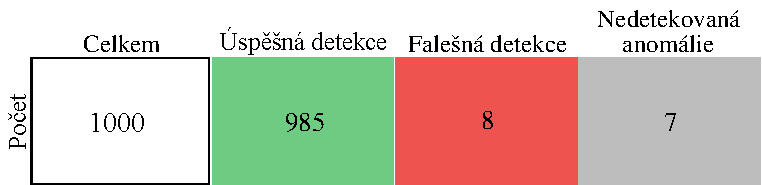
\includegraphics[width=0.83\textwidth]{obrazky/result-matrix.pdf}
    \caption{Číselné výsledky testu detekce anomálií nad náhodnými datasety}
    \label{matice-vysledku-img}
\end{figure}

V~8 datasetech došlo k~falešné detekci anomálie. Celkem 5 případů spočívalo v~klasifikaci přirozených outlierů jako anomálie. Ve zbylých 3 byly za~anomálie považovány shluky jako na~obrázku~\ref{chybne-nalezena-anomalie-img}.

\begin{figure}[hbt]
    \centering
    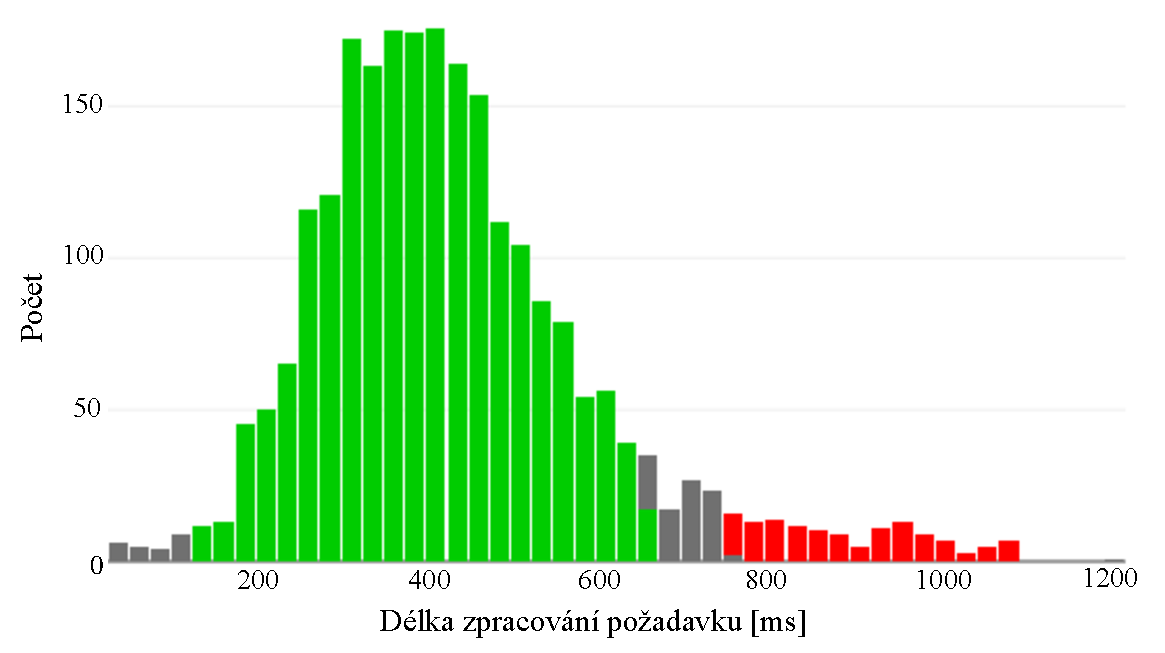
\includegraphics[width=0.9\textwidth]{obrazky/testovani-false-anomaly.pdf}
    \caption{V~těchto datech se chybně nalezla anomálie. Outliery byly zřejmě dostatečně blízko sebe na~vytvoření širokého, řídkého a rovnoměrného shluku, jenž se však v~celkovém kontextu anomálně nechová.}
    \label{chybne-nalezena-anomalie-img}
\end{figure}

Pouze v~7 případech se anomálii nepodařilo detekovat. Jen ve~4 z~nich však byla anomálie naprosto zřetelná. V~ostatních se jednalo o~sporné situace podobné obrázku~\ref{nenalezena-anomalie-img}, kde je spíše věcí názoru, jestli by se o~anomálii jednat mělo, či ještě ne.

\begin{figure}[!hbt]
    \centering
    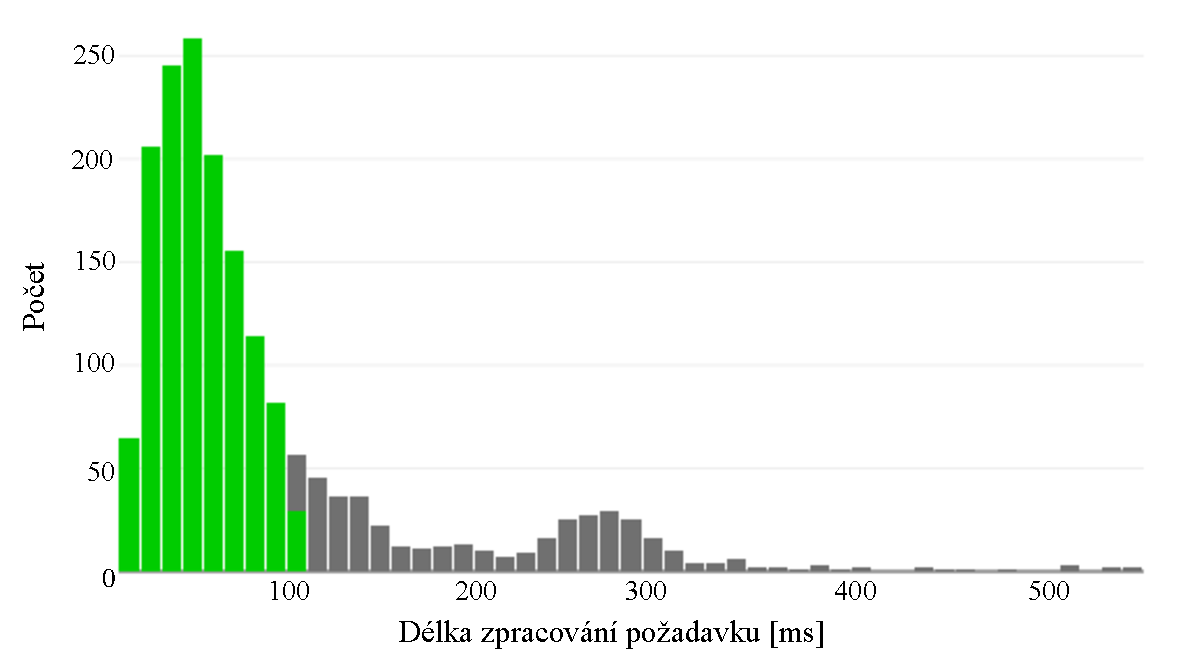
\includegraphics[width=0.9\textwidth]{obrazky/testovani-unrecognized-anomaly.pdf}
    \caption{Výkyv v~datech nebyl rozpoznán jako anomálie.}
    \label{nenalezena-anomalie-img}
\end{figure}

Dále se při~úspěšné detekci 9krát stalo, že k~sobě anomálie zahrnula i okolní data, jež by do~ní patřit neměla. Toto zobrazuje obrázek~\ref{prilis-siroka-anomalie-img}. Byť se jedná o~nepřesnost, přímo za~chybu se to nepovažuje, neboť anomálie detekována byla a uživatel by již neměl problém si situaci interpretovat.

\begin{figure}[!hbt]
    \centering
    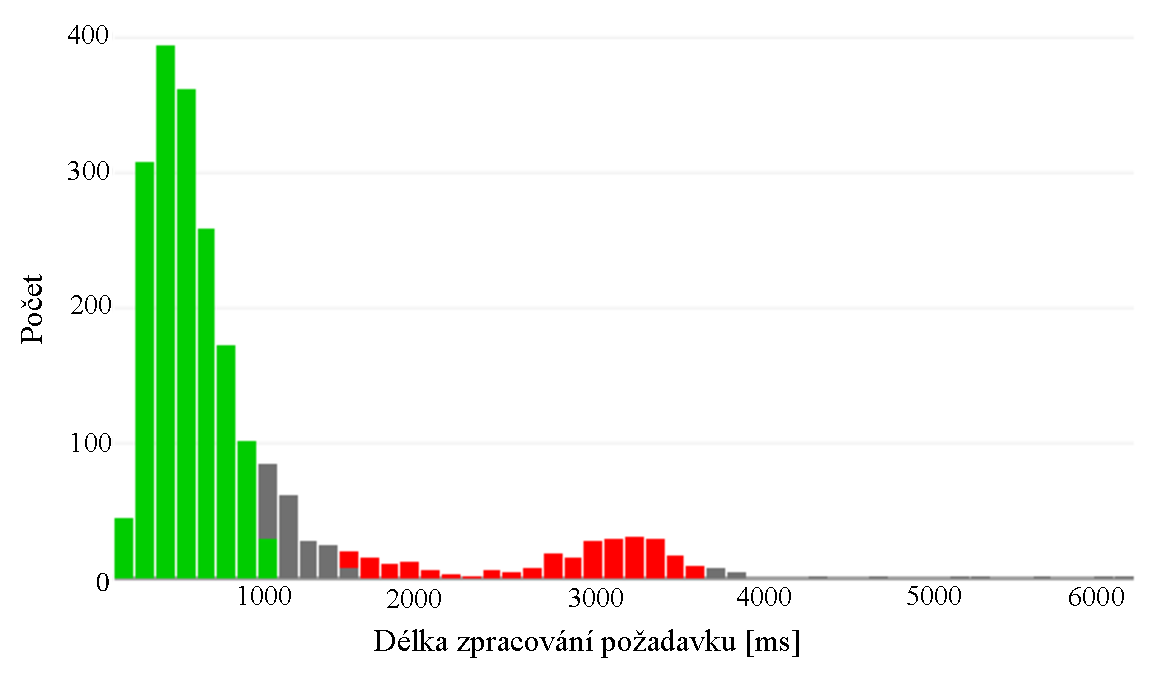
\includegraphics[width=0.9\textwidth]{obrazky/testovani-too-wide-anomaly.pdf}
    \caption{Anomálie obsahuje i okolní data, která již nejsou přímo součástí shluku.}
    \label{prilis-siroka-anomalie-img}
\end{figure}

Výsledek si lze vyložit velmi pozitivně. Celkových~985 správných detekcí z~1000 dělá úspěšnost 98.5~\%, což je velmi uspokojivé. Dále pokud by se bral v~potaz parametr tolerance pro~potlačení anomálií blízko dat, jenž bude v~RQA zcela jistě použit, přirozené outliery by se za~anomálie nikdy neklasifikovaly. To by v~tomto případě zvýšilo počet správných detekcí na~990 a úspěšnost na~99~\%. Kdyby se navíc nebraly v~potaz sporné anomálie, tak~990 správných detekcí z~997 dělá úspěšnost zaokrouhleně~99.3~\%.

\section{Testování detekce anomálií v~chybovosti požadavků}
Testování této funkcionality se ukázalo být celkem jednoduché. Vzhledem k~tomu, že se jedná pouze o~porovnání poměrů počtů chyb mezi dvěma datasety, stačilo ověřit jen několik specifických případů. Nejprve se vytvořil referenční dataset obsahující~70~\% požadavků bez chyb,~20~\% s~1 chybou a zbylých~10~\% se~2 chybami. Dále se testovalo, zda-li se anomálie detekuje, bude-li vše v~mezích. Vygenerovalo se několik datasetů takovým způsobem, aby nebyl nikdy nepřekročen rozdíl~10~\% u~některého počtu chyb, tedy s~60-80~\% požadavků bez chyb,~10-30~\% s~1 chybou a~0-20~\% se~2 chybami. Anomálie nebyla nikdy detekována.

Dále se testovaly anomální situace. První je překročení dané meze. Vygenerovaly se tedy datasety obsahující více než~80~\% nebo méně než~60~\% požadavků bez chyb a podobně i u~ostatních počtů chyb. Druhým typem anomálie je doposud neviděný počet chyb. Proto byly vytvořeny datasety s~požadavky se~3 i více chybami, ať už v~rámci anomální meze, nebo ne. V~obou případech se jedná o~anomálii. Všechny požadované anomální stavy byly rozeznány.

\section{Vyhodnocení dosažených výsledků}
Na~základě výsledků testů sekce~\ref{testovani-delka-pozadavku} lze dospět k~závěru, že detekce anomálií v~délkách zpracování požadavků funguje velmi dobře. Úspěšnost přesahující 98~\% je toho zjevným důkazem. Těchto výsledků bylo dosaženo i navzdory požadavku na~obecnost detekce. Řešení navíc není zcela uzavřené a umožňuje uživateli nastavovat toleranci pro~anomálie, ať už v~její velikosti nebo pozici.

Návrh detekce s~ohledem na~obecnost dat však nepopiratelně zapříčiňuje nepřesnosti. Jednou z~nich je nespolehlivé rozpoznání okrajů platných dat, čímž se z~nich již stávají outliery. Další je, že anomální shluky občas neobsahují vše, co by měly, nebo naopak mají přesah do~dat, jež by do~nich již patřit neměly. Někdy zase obecné parametry nedostačují pro~kvalitní shlukování a anomálii se nepodaří detekovat. S~rostoucími požadavky na~obecnost klesá přesnost, a~proto je řešení kompromisem, jenž se části přesnosti musel vzdát.

Detekce anomálií v~chybách během požadavků nevyužívá žádné specifické algoritmy strojového učení, nýbrž jen statistické výpočty. Bude tedy vždy vykazovat stejné výsledky dle definovaných parametrů. Všechny specifikované anomální případy dokáže rozpoznat, a~tak jestli nedojde k~nepředpokládané situaci, bude vždy pracovat správně.

Výsledky jsou pozitivně vnímány i firmou Y~Soft, jejíž posudek je přiložen v~příloze~\ref{priloha-D}. Způsob provedení i funkčnost plně splňují jejich požadavky. Z~technického hlediska jsou spokojeni především se snadným zahrnutím mikroslužeb do~detekce anomálií pomocí instalace rozšíření a implementací na~platformě .NET.